
\chapter{Team Coordination and Project Management}
\label{chapter:teamplan}

Effective communication is the cornerstone of successful software development, especially in multidisciplinary teams. A structured \textbf{Team Communication Plan} ensures that all members remain aligned, informed, and coordinated toward shared objectives.

This chapter presents the communication strategies and project management practices adopted throughout SPLASH's development. These include the selection of collaboration tools, scheduling methodologies, team structure, and risk mitigation strategies. Together, they form a robust framework to support the project's lifecycle—from initial planning to final deployment.

\section{Communication Tools and Platforms}
\label{section:comunication_tools}

\begin{itemize}
    \item \textbf{GitHub:} Used for version control and collaborative development. It serves as the central repository for source code, issue tracking, and code review.
    \item \textbf{OneDrive \& Overleaf:} Used for collaborative documentation. These tools allow for real-time editing and maintain a consistent version history of all written deliverables.
    \item \textbf{Jira:} Employed for agile project management, sprint planning, and milestone tracking. Provides an overview of tasks and responsibilities.
    \item \textbf{Discord:} Chosen for synchronous communication, including voice calls, video meetings, and chat. Enables both scheduled and informal interactions.
\end{itemize}

\newpage

\section{Schedule and Meetings}
\label{section:schedule_meetings}

\textbf{Excel} was used to coordinate individual availabilities and to schedule regular team meetings and supervisor check-ins. This tool enabled effective time management and ensured team-wide alignment, as illustrated in Figure~\ref{fig:schedule}.

\begin{figure}[H]
      \centering
      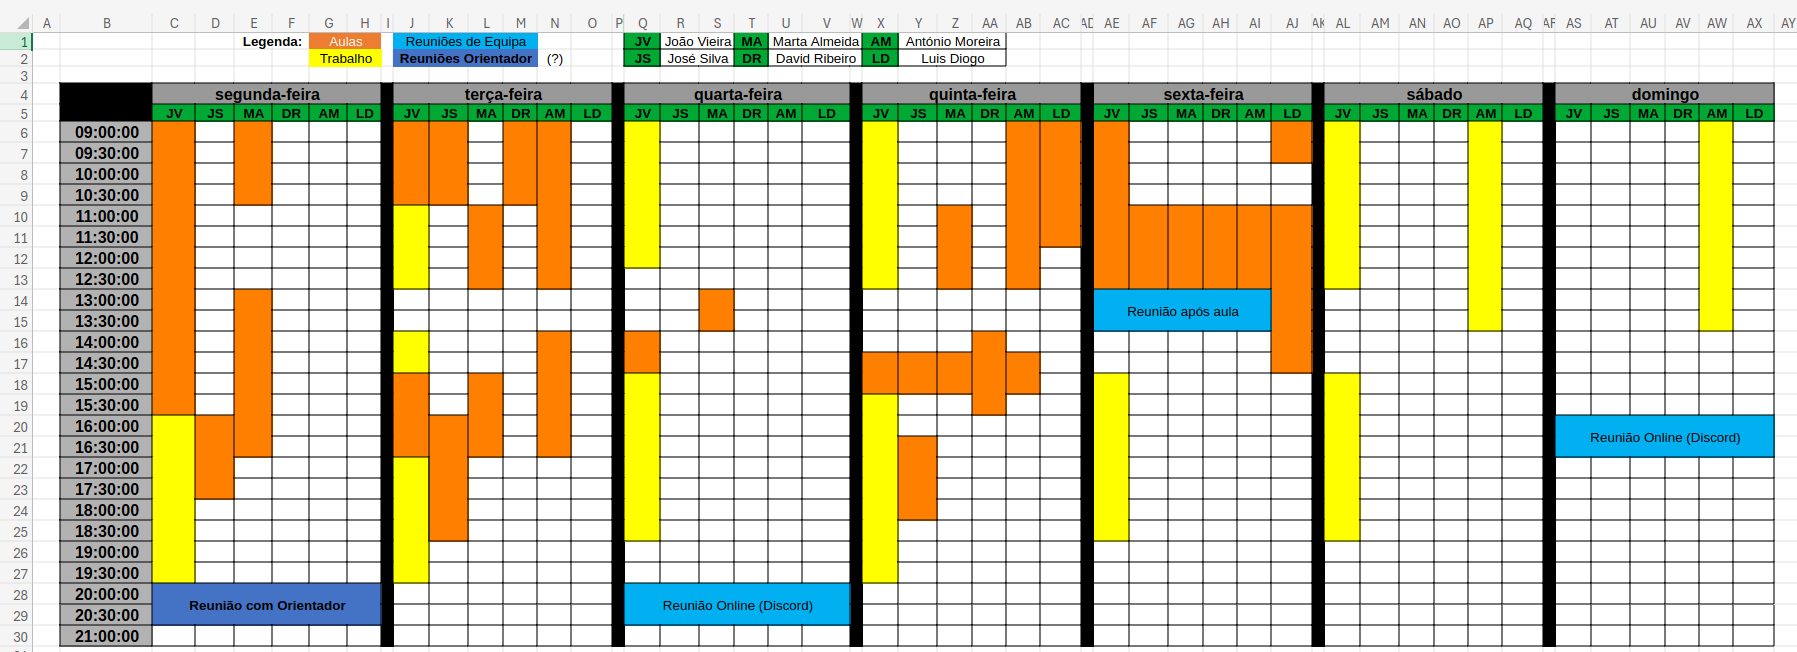
\includegraphics[width=16cm]{figs/team_schedule_1.png}
      \caption{Team schedule and meeting planner implemented in Excel, showing member availability, scheduled meetings, and project milestones for the first semester}
      \label{fig:schedule1}
\end{figure}

\begin{figure}[H]
      \centering
      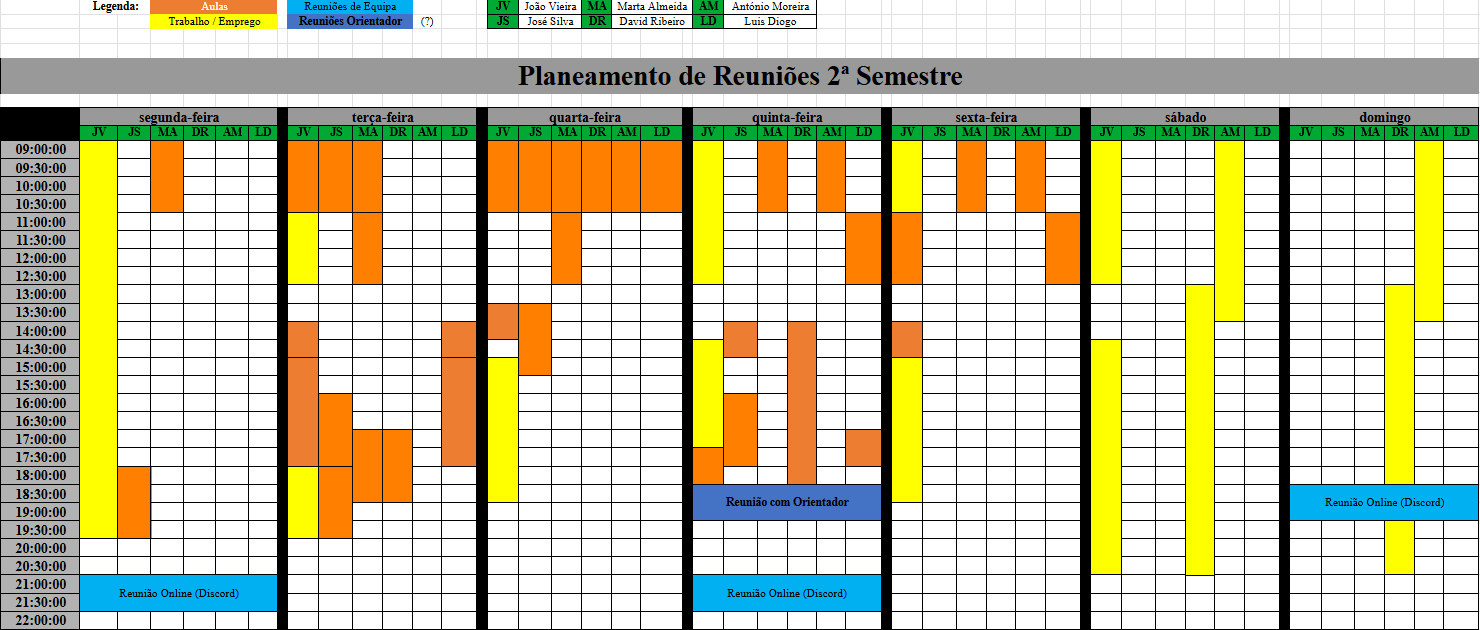
\includegraphics[width=16cm]{figs/team_schedule_2.png}
      \caption{Team schedule and meeting planner implemented in Excel, showing member availability, scheduled meetings, and project milestones for the second semester}
      \label{fig:schedule2}
\end{figure}

\section{Team Structure and Roles}
\label{section:team_structure}

Effective project execution relies heavily on a well-defined team structure with clear responsibilities. This section outlines the adopted framework, designed to optimize workflow and ensure comprehensive coverage of project needs.

\newpage

\subsection{SCRUM Master}
\label{subsec:scrum_master}

João Vieira was designated as the \textit{SCRUM Master}, responsible for:

\begin{itemize}
    \item Facilitating the SCRUM process
    \item Ensuring adherence to SCRUM principles
    \item Removing obstacles to team progress
    \item Fostering a culture of continuous improvement
\end{itemize}

\subsection{Sub-teams}
\label{subsec:sub_teams}

To leverage team strengths, members were grouped into three specialized sub-teams:

\subsubsection{Frontend Development Team}
\begin{itemize}
    \item \textbf{Team Leader:} José Silva 
    \item \textbf{Members:} José Silva \& Antonio Moreira
    \item \textbf{Responsibilities:}
    \begin{itemize}
        \item UI design and implementation
        \item Responsive layout creation
        \item UX optimization
        \item Integration with backend APIs
    \end{itemize}
\end{itemize}

\subsubsection{Backend Development Team}
\begin{itemize}
    \item \textbf{Team Leader:} João Vieira 
    \item \textbf{Members:} João Vieira
    \item \textbf{Responsibilities:}
    \begin{itemize}
        \item Server-side logic and database design
        \item API development
        \item Performance optimization
    \end{itemize}
\end{itemize}

\subsubsection{Data Team}
\begin{itemize}
    \item \textbf{Team Leader:}  Marta Almeida
    \item \textbf{Members:}  Marta Almeida \& David  Ribeiro
    \item \textbf{Responsibilities:}
    \begin{itemize}
        \item Validation and processing of quiz results submitted by lifeguards
        \item Planning, execution, and storage of user testing data
        \item Providing technical support to other teams regarding data-related matters
    \end{itemize}
\end{itemize}
\subsubsection{Hardware Development Team}
\begin{itemize}
    \item \textbf{Team Leader:}  Luis Diogo
    \item \textbf{Members:}  Luis Diogo
    \item \textbf{Responsibilities:}
    \begin{itemize}
        \item Develop embedded firmware
        \item Integrating devices with the SPLASH ecosystem 
    \end{itemize}
\end{itemize}


\section{Risk Analysis and Mitigation Strategies}
\label{section:risk_analisys_mitigation_strategies}

The implementation of SPLASH involves technological, environmental, and human-related risks. These must be addressed to ensure system reliability and user safety.

\begin{itemize}
    \item \textbf{Hardware and Connectivity Failures:} Devices such as GPS wristbands or communication tablets may malfunction or lose connectivity. This can be mitigated through pre-deployment testing, scheduled maintenance, and having redundant devices available.

    \item \textbf{Environmental Conditions:} Weather-related events (e.g., high winds, salt exposure) may affect equipment performance. Selecting durable, weather-resistant hardware and establishing operational contingency protocols can reduce these risks.

    \item \textbf{Human Error and Technological Adoption:} Some users may struggle with adapting to new tools. This risk is mitigated by ensuring the interface remains user-friendly and providing training sessions to lifeguards and supervisors.
\end{itemize}

\section{Conclusion}
In summary, the project's success depended not only on technical development but also on structured communication and clearly defined responsibilities. The use of collaborative tools, agile methodologies, and proactive risk management contributed significantly to the team's cohesion and overall project quality.





%%
%\begin{thebibliography}{9}

%\bibitem{infopraia1} 
%Info Praia.
%\textit{Informação sobre as praias portuguesas.}
%Disponível em: \url{https://infopraia.apambiente.pt/about/}, %acedido em 12/11/2024.

%\bibitem{infopraia2} 
%Sistema Nacional de Informação de Recursos Hídricos.
%\textit{Info Praia - Informações detalhadas sobre praias.}
%Disponível em: \url{https://snirh.apambiente.pt/index.php?%idMain=1&idItem=2.1}, acedido em 12/11/2024.

%\bibitem{praia5g1} 
%Costa da Caparica: Primeira Praia com Cobertura 5G.
%\textit{SAPO Tek - Notícias sobre telecomunicações.}
%Disponível em: \url{https://tek.sapo.pt/noticias/telecomunicacoes/%artigos/costa-da-caparica-e-a-primeira-praia-portuguesa-com-%cobertura-5g}, acedido em 14/11/2024.

%\bibitem{praia5g2} 
%NOS.
%\textit{Primeira Praia 5G - Casos de inovação.}
%Disponível em: \url{https://www.nos.pt/5g/5g-em-acao/casos-de-%inovacao/primeira-praia-5g}, acedido em 14/11/2024.

%\end{thebibliography}
%\end{document}